\documentclass[12pt, titlepage]{article}

\usepackage{fullpage}
\usepackage[round]{natbib}
\usepackage{multirow}
\usepackage{booktabs}
\usepackage{tabularx}
\usepackage{graphicx}
\usepackage{float}
\usepackage{hyperref}
\hypersetup{
    colorlinks,
    citecolor=blue,
    filecolor=black,
    linkcolor=red,
    urlcolor=blue
}

%% Comments

\usepackage{color}

\newif\ifcomments\commentstrue %displays comments
%\newif\ifcomments\commentsfalse %so that comments do not display

\ifcomments
\newcommand{\authornote}[3]{\textcolor{#1}{[#3 ---#2]}}
\newcommand{\todo}[1]{\textcolor{red}{[TODO: #1]}}
\else
\newcommand{\authornote}[3]{}
\newcommand{\todo}[1]{}
\fi

\newcommand{\wss}[1]{\authornote{blue}{SS}{#1}} 
\newcommand{\plt}[1]{\authornote{magenta}{TPLT}{#1}} %For explanation of the template
\newcommand{\an}[1]{\authornote{cyan}{Author}{#1}}

%% Common Parts

\newcommand{\progname}{Damped Harmonic Ocsillator} % PUT YOUR PROGRAM NAME HERE
\newcommand{\authname}{
\\ Muhammad Waqar Ul Hassan Awan
} % AUTHOR NAMES                  

\usepackage{hyperref}
    \hypersetup{colorlinks=true, linkcolor=blue, citecolor=blue, filecolor=blue,
                urlcolor=blue, unicode=false}
    \urlstyle{same}
                                


\newcounter{acnum}
\newcommand{\actheacnum}{AC\theacnum}
\newcommand{\acref}[1]{AC\ref{#1}}

\newcounter{ucnum}
\newcommand{\uctheucnum}{UC\theucnum}
\newcommand{\uref}[1]{UC\ref{#1}}

\newcounter{mnum}
\newcommand{\mthemnum}{M\themnum}
\newcommand{\mref}[1]{M\ref{#1}}

\begin{document}

\title{Module Guide for \progname{}} 
\author{\authname}
\date{\today}

\maketitle

\pagenumbering{roman}

\section{Revision History}

\begin{tabularx}{\textwidth}{p{3cm}p{2cm}X}
\toprule {\bf Date} & {\bf Version} & {\bf Notes}\\
\midrule
18 Mar, 2024 & 1.0 & Initial MG documentation\\
\bottomrule
\end{tabularx}

\newpage

\section{Reference Material}

This section records information for easy reference.

\subsection{Abbreviations and Acronyms}

\renewcommand{\arraystretch}{1.2}
\begin{tabular}{l l} 
  \toprule		
  \textbf{symbol} & \textbf{description}\\
  \midrule 
  SRS & Software Requirement Specification\\
  ODE & Ordinary Differential Equation\\
  DE & Differential Equation\\
  DHO & Damped Harmonic Oscillator\\
  SHM & Simple Harmonic Motion\\
  \bottomrule
\end{tabular}\\

\newpage

\tableofcontents

\listoftables

\listoffigures

\newpage

\pagenumbering{arabic}

\section{Introduction}

Decomposing a system into modules is a commonly accepted approach to developing
software.  A module is a work assignment for a programmer or programming
team~\citep{ParnasEtAl1984}.  We advocate a decomposition
based on the principle of information hiding~\citep{Parnas1972a}.  This
principle supports design for change, because the ``secrets'' that each module
hides represent likely future changes.  Design for change is valuable in SC,
where modifications are frequent, especially during initial development as the
solution space is explored.  

Our design follows the rules layed out by \citet{ParnasEtAl1984}, as follows:
\begin{itemize}
\item System details that are likely to change independently should be the
  secrets of separate modules.
\item Each data structure is implemented in only one module.
\item Any other program that requires information stored in a module's data
  structures must obtain it by calling access programs belonging to that module.
\end{itemize}

After completing the first stage of the design, the Software Requirements
Specification (SRS), the Module Guide (MG) is developed~\citep{ParnasEtAl1984}. The MG
specifies the modular structure of the system and is intended to allow both
designers and maintainers to easily identify the parts of the software.  The
potential readers of this document are as follows:

\begin{itemize}
\item New project members: This document can be a guide for a new project member
  to easily understand the overall structure and quickly find the
  relevant modules they are searching for.
\item Maintainers: The hierarchical structure of the module guide improves the
  maintainers' understanding when they need to make changes to the system. It is
  important for a maintainer to update the relevant sections of the document
  after changes have been made.
\item Designers: Once the module guide has been written, it can be used to
  check for consistency, feasibility, and flexibility. Designers can verify the
  system in various ways, such as consistency among modules, feasibility of the
  decomposition, and flexibility of the design.
\end{itemize}

The rest of the document is organized as follows. Section
\ref{SecChange} lists the anticipated and unlikely changes of the software
requirements. Section \ref{SecMH} summarizes the module decomposition that
was constructed according to the likely changes. Section \ref{SecConnection}
specifies the connections between the software requirements and the
modules. Section \ref{SecMD} gives a detailed description of the
modules. Section \ref{SecTM} includes two traceability matrices. One checks
the completeness of the design against the requirements provided in the SRS. The
other shows the relation between anticipated changes and the modules. Section
\ref{SecUse} describes the use relation between modules.

\section{Anticipated and Unlikely Changes} \label{SecChange}

This section lists possible changes to the system. According to the likeliness
of the change, the possible changes are classified into two
categories. Anticipated changes are listed in Section \ref{SecAchange}, and
unlikely changes are listed in Section \ref{SecUchange}.

\subsection{Anticipated Changes} \label{SecAchange}

Anticipated changes are the source of the information that is to be hidden
inside the modules. Ideally, changing one of the anticipated changes will only
require changing the one module that hides the associated decision. The approach
adapted here is called design for
change.

\begin{description}
\item[\refstepcounter{acnum} \actheacnum \label{acInitInput}:] The format of the initial input data.
\item[\refstepcounter{acnum} \actheacnum \label{acInputParams}:]The format of the input parameters.
\item[\refstepcounter{acnum} \actheacnum \label{acInputConstraints}:] The constraints on the input parameters.
\item[\refstepcounter{acnum} \actheacnum \label{acFinalOutput}:] The format of the final output data.
\item[\refstepcounter{acnum} \actheacnum \label{acUserInterface}:] As user feedback is collected and as the software finds use in broader contexts, adjustments to the user interface may be necessary to enhance usability, accessibility, and user experience.
\item[\refstepcounter{acnum} \actheacnum \label{acOutputPlot}:] How the plotting of the output is implemented.
\item[\refstepcounter{acnum} \actheacnum \label{acCalcControl}:] The overall control of the calculation.
\item[\refstepcounter{acnum} \actheacnum \label{acFutureDev}:] Future developments might necessitate the inclusion of more complex systems such as coupled oscillators or multidimensional oscillatory systems.
\end{description}

\subsection{Unlikely Changes} \label{SecUchange}

The module design should be as general as possible. However, a general system is
more complex. Sometimes this complexity is not necessary. Fixing some design
decisions at the system architecture stage can simplify the software design. If
these decision should later need to be changed, then many parts of the design
will potentially need to be modified. Hence, it is not intended that these
decisions will be changed.

\begin{description}
\item[\refstepcounter{ucnum} \uctheucnum \label{ucIODevices}:] Input/Output devices (Input: File and/or Keyboard, Output: File, Memory, and/or
Screen).
\item[\refstepcounter{ucnum} \uctheucnum \label{ucMathPrinciples}:] The fundamental physics and mathematics governing harmonic oscillators are well-established. Significant changes to these principles are unlikely and would fundamentally alter the nature of the software.
\item[\refstepcounter{ucnum} \uctheucnum \label{ucProgLanguage}:] The selection of the programming language and core libraries is based on their ability to handle the computational requirements and maintainability of the software. While updates and minor changes to dependencies are expected, a complete shift is unlikely due to the substantial effort involved in rewriting and revalidating the software.
\item[\refstepcounter{ucnum} \uctheucnum \label{ucProgLanguage}:] The selection of the programming language and core libraries is based on their ability to handle the computational requirements and maintainability of the software. While updates and minor changes to dependencies are expected, a complete shift is unlikely due to the substantial effort involved in rewriting and revalidating the software.
\item[\refstepcounter{ucnum} \uctheucnum \label{ucStandaloneApp}:] The software is designed as a specific solution to modeling harmonic oscillators with damping. Changing its operational mode from a standalone application to an integrated module within a larger system, or vice versa, would require a significant architectural change.
\end{description}

\section{Module Hierarchy} \label{SecMH}

This section provides an overview of the module design. Modules are summarized
in a hierarchy decomposed by secrets in Table \ref{TblMH}. The modules listed
below, which are leaves in the hierarchy tree, are the modules that will
actually be implemented. Modules are numbered
by M followed by a number.

\begin{description}
\item [\refstepcounter{mnum} \mthemnum \label{mHH}:] Hardware-Hiding Module
\item [\refstepcounter{mnum} \mthemnum \label{mDI}:] Data Input Module
\item [\refstepcounter{mnum} \mthemnum \label{mPI}:] Parameter Input Module
\item [\refstepcounter{mnum} \mthemnum \label{mCE}:] Calculation Engine Module
\item [\refstepcounter{mnum} \mthemnum \label{mOM}:] Output Module
\item [\refstepcounter{mnum} \mthemnum \label{mUIM}:] User Interface Module
\item [\refstepcounter{mnum} \mthemnum \label{mPVM}:] Plotting and Visualization Module
\item [\refstepcounter{mnum} \mthemnum \label{mODEM}:] ODE Solver Module
\end{description}

Note that \mref{mHH} is a commonly used module and is already implemented by the operating system.  It will not be reimplemented.  Similarly, \mref{mPVM} and  \mref{mODEM} are already available in Python/React and will not be reimplemented.


\begin{table}[h!]
\centering
\begin{tabular}{p{0.3\textwidth} p{0.6\textwidth}}
\toprule
\textbf{Level 1} & \textbf{Level 2}\\
\midrule

{Hardware-Hiding Module} & \mref{mHH} \\
\midrule

\multirow{5}{0.3\textwidth}{Behaviour-Hiding Module} & \mref{mDI}\\
& \mref{mPI}\\
& \mref{mCE}\\
& \mref{mOM}\\
& \mref{mUIM}\\
\midrule

\multirow{2}{0.3\textwidth}{Software Decision Module} & \mref{mPVM}\\
& \mref{mODEM}\\
\bottomrule

\end{tabular}
\caption{Module Hierarchy}
\label{TblMH}
\end{table}

\section{Connection Between Requirements and Design} \label{SecConnection}

The design of the system is intended to satisfy the requirements developed in
the SRS. In this stage, the system is decomposed into modules. The connection
between requirements and modules is listed in Table~\ref{TblRT}.

\section{Module Decomposition} \label{SecMD}

Modules are decomposed according to the principle of ``information hiding''
proposed by \citet{ParnasEtAl1984}. The \emph{Secrets} field in a module
decomposition is a brief statement of the design decision hidden by the
module. The \emph{Services} field specifies \emph{what} the module will do
without documenting \emph{how} to do it. For each module, a suggestion for the
implementing software is given under the \emph{Implemented By} title. If the
entry is \emph{OS}, this means that the module is provided by the operating
system or by standard programming language libraries.  \emph{\progname{}} means the
module will be implemented by the \progname{} software.

Only the leaf modules in the hierarchy have to be implemented. If a dash
(\emph{--}) is shown, this means that the module is not a leaf and will not have
to be implemented.

\subsection{Hardware Hiding Modules (\mref{mHH})}

\begin{description}
\item[Secrets:]The data structure and algorithm used to implement the virtual
  hardware.
\item[Services:]Serves as a virtual hardware used by the rest of the
  system. This module provides the interface between the hardware and the
  software. So, the system can use it to display outputs or to accept inputs.
\item[Implemented By:] OS
\end{description}

\subsection{Behaviour-Hiding Module}

\begin{description}
\item[Secrets:]The contents of the required behaviours.
\item[Services:]Includes programs that provide externally visible behaviour of
  the system as specified in the \href{https://github.com/WaqarAwan376/Damped_Harmonic_Oscillator-CAS741/tree/main/docs/SRS}{software requirements specification (SRS)}
  documents. This module serves as a communication layer between the
  hardware-hiding module and the software decision module. The programs in this
  module will need to change if there are changes in the SRS.
\item[Implemented By:] --
\end{description}

\subsubsection{Data Input Module (\mref{mDI})}

\begin{description}
\item[Secrets:]The format and validation rules for the data entered by the user.
\item[Services:]Validates and transforms user input into a standardized format for processing by the calculation engine. Ensures that all inputs meet the constraints and formats expected by the system.
\item[Implemented By:] Damped Harmonic Oscillator
\item[Type of Module:] Library
\end{description}

\subsubsection{Parameter Input Module (\mref{mPI})}

\begin{description}
\item[Secrets:]The structure and validation criteria for simulation parameters.
\item[Services:]Processes and validates the parameters specific to the damped harmonic oscillator simulation, such as mass, spring constant, damping coefficients, etc.
\item[Implemented By:] Damped Harmonic Oscillator
\item[Type of Module:] Library
\end{description}

\subsubsection{Calculation Engine Module (\mref{mCE})}

\begin{description}
\item[Secrets:]The algorithms that implement the mathematical models of the damped harmonic oscillator.
\item[Services:]Performs the core calculations based on input parameters and models, generating the dynamics of the oscillator over time.
\item[Implemented By:] Damped Harmonic Oscillator
\item[Type of Module:] Library
\end{description}

\subsubsection{Output Module (\mref{mOM})}

\begin{description}
\item[Secrets:]The data structure and algorithms used to format simulation results for output.
\item[Services:]Transforms calculation results into various output formats (e.g., graphical, textual) for user interpretation.
\item[Implemented By:] Damped Harmonic Oscillator
\item[Type of Module:] Library
\end{description}

\subsubsection{User Interface Module (\mref{mUIM})}

\begin{description}
\item[Secrets:]The design and logic for the software's user interface.
\item[Services:]Provides the graphical or command-line interface through which users interact with the software, including inputting parameters and viewing results.
\item[Implemented By:] Damped Harmonic Oscillator
\item[Type of Module:] Library
\end{description}


\subsection{Software Decision Module}

\begin{description}
\item[Secrets:] The design decision based on mathematical theorems, physical
  facts, or programming considerations. The secrets of this module are
  \emph{not} described in the SRS.
\item[Services:] Includes data structure and algorithms used in the system that
  do not provide direct interaction with the user. 
\item[Implemented By:] --
\end{description}

\subsubsection{Plotting and Visualization Module (\mref{mPVM})}

\begin{description}
\item[Secrets:]The algorithms and libraries used to generate visual representations of the simulation results.
\item[Services:]Creates charts, graphs, and animations to visually depict the behavior of the damped harmonic oscillator based on the simulation outcomes.
\item[Implemented By:] ReactJS
\item[Type of Module:] Library
\end{description}

\subsubsection{ODE Solver Module (\mref{mODEM})}

\begin{description}
\item[Secrets:]The numerical methods and algorithms for solving ordinary differential equations (ODEs) that describe the motion of the damped harmonic oscillator.
\item[Services:]Provides the computational backbone for accurately solving the equations of motion under various conditions and damping models.
\item[Implemented By:] Python
\item[Type of Module:] Library
\end{description}

\section{Traceability Matrix} \label{SecTM}

This section shows two traceability matrices: between the modules and the
requirements and between the modules and the anticipated changes.

\begin{table}[H]
\centering
\begin{tabular}{p{0.2\textwidth} p{0.6\textwidth}}
\toprule
\textbf{Req.} & \textbf{Modules}\\
\midrule
R1 & \mref{mDI}, \mref{mPI}\\
R2 & \mref{mUIM}\\
R3 & \mref{mCE}, \mref{mOM}\\
R4 & \mref{mCE}\\
R5 & \mref{mOM}, \mref{mPVM}\\
NFR1 & \mref{mCE}\\
NFR1 & \mref{mUIM}\\
NFR1 & Depends on the nature of the change\\
NFR1 & \mref{mHH}\\
\bottomrule
\end{tabular}
\caption{Trace Between Requirements and Modules}
\label{TblRT}
\end{table}

\begin{table}[H]
\centering
\begin{tabular}{p{0.2\textwidth} p{0.6\textwidth}}
\toprule
\textbf{AC} & \textbf{Modules}\\
\midrule
\acref{acInitInput} & \mref{mDI}\\
\acref{acInputParams} & \mref{mPI}\\
\acref{acInputConstraints} & \mref{mPI}\\
\acref{acFinalOutput} & \mref{mOM}\\
\acref{acUserInterface} & \mref{mUIM}\\
\acref{acOutputPlot} & \mref{mPVM}\\
\acref{acCalcControl} & \mref{mCE}\\
\acref{acFutureDev} & \mref{mCE}\\
\bottomrule
\end{tabular}
\caption{Trace Between Anticipated Changes and Modules}
\label{TblACT}
\end{table}

\section{Use Hierarchy Between Modules} \label{SecUse}

In this section, the uses hierarchy between modules is
provided. \citet{Parnas1978} said of two programs A and B that A {\em uses} B if
correct execution of B may be necessary for A to complete the task described in
its specification. That is, A {\em uses} B if there exist situations in which
the correct functioning of A depends upon the availability of a correct
implementation of B.  Figure \ref{FigUH} illustrates the use relation between
the modules. It can be seen that the graph is a directed acyclic graph
(DAG). Each level of the hierarchy offers a testable and usable subset of the
system, and modules in the higher level of the hierarchy are essentially simpler
because they use modules from the lower levels.

\begin{figure}[h!]
\centering
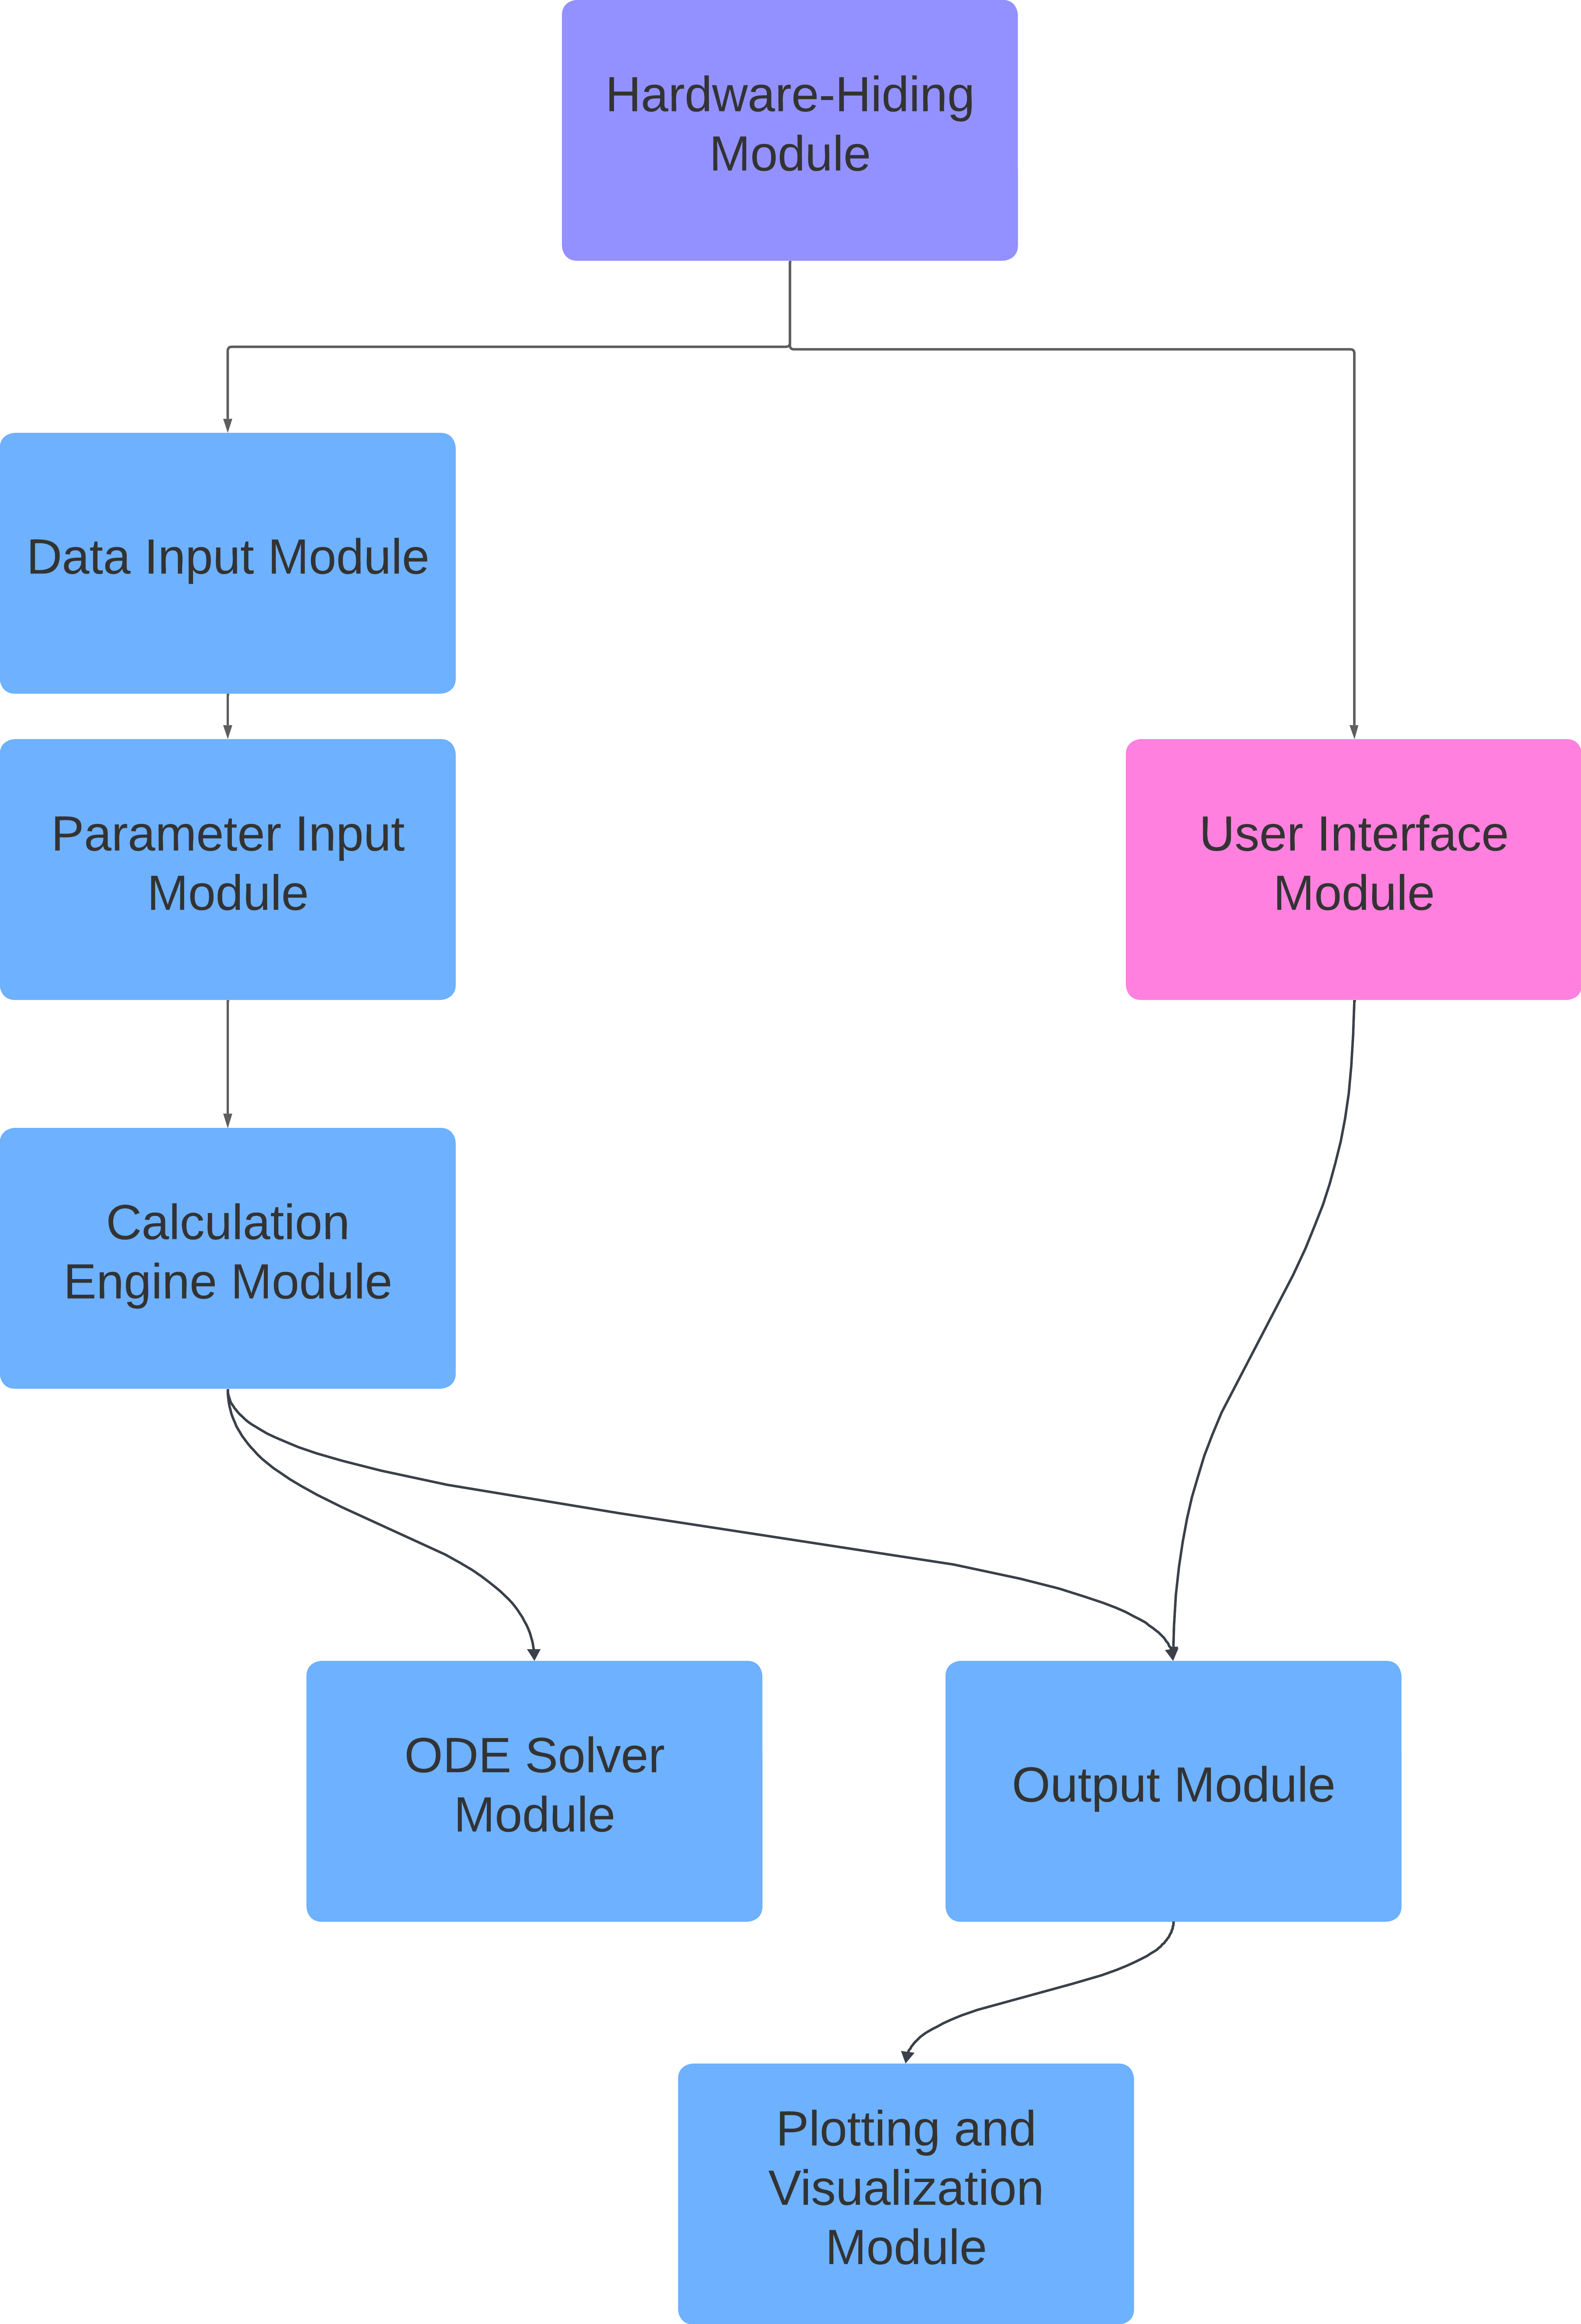
\includegraphics[width=0.7\textwidth]{hierarchy.png}
\caption{Use hierarchy among modules}
\label{FigUH}
\end{figure}

\section{User Interfaces}

Following is a tentative design for the Damped harmonic oscillator simulation.

\begin{figure}[h!]
  \centering
  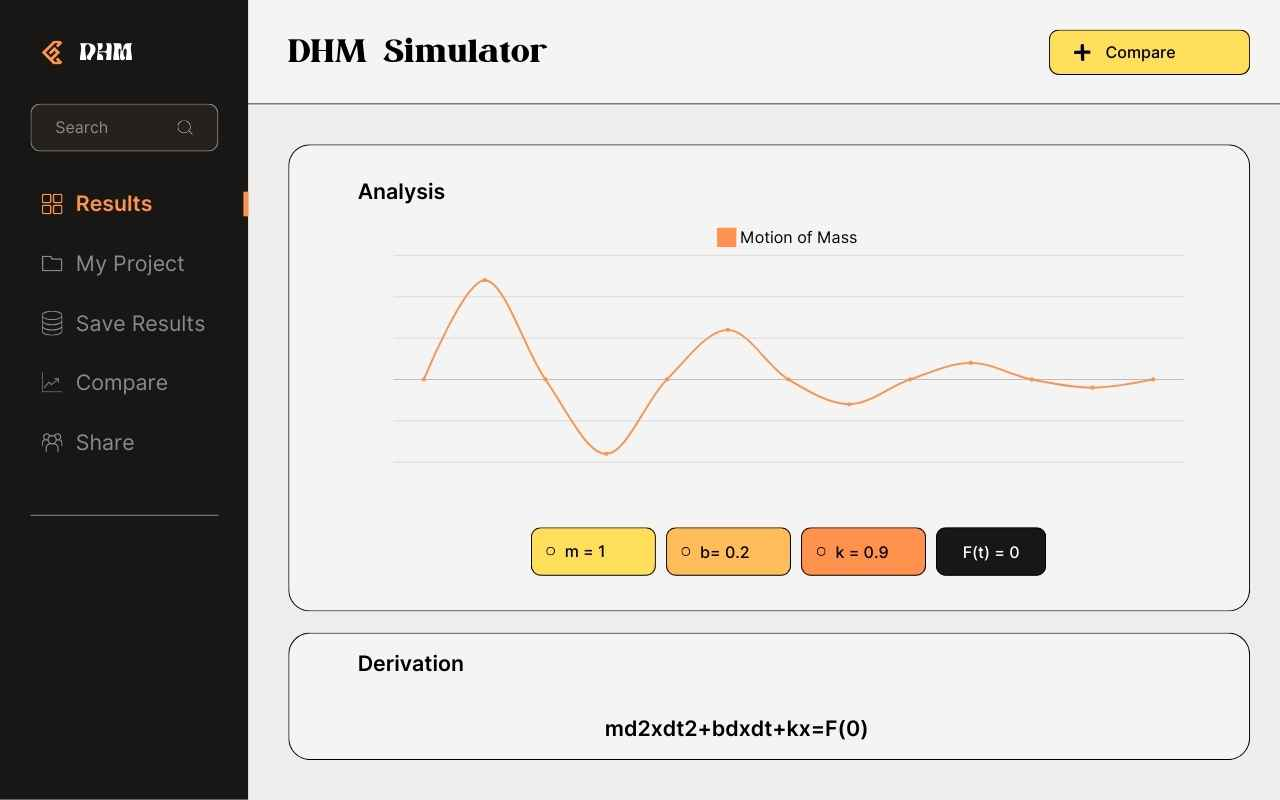
\includegraphics[width=0.7\textwidth]{UI.jpg}
  \caption{Tentative Design}
  \label{FigUI}
\end{figure}

\section{Timeline}


Table displays the timeline for the development of each module and its respective developer.

\begin{table}[H]
\centering
\begin{tabular}{p{0.2\textwidth} p{0.4\textwidth}  p{0.4\textwidth}}
\toprule
 \textbf{Modules} & \textbf{Time} & \textbf{Responsible} \\
\midrule
Frontend& 20 March - 03 April & Waqar\\
Backend & 24 March - 03 April & Waqar\\
\bottomrule
\end{tabular}
\caption{Timeline}
\end{table}

\bibliographystyle {plainnat}
\bibliography{../../../refs/References}

\newpage{}

\end{document}